
\FloatBarrier

\chapter{The bit stream layer}
\label{cha:bitstream}

In this chapter, we describe the intermediate abstractions levels the
packet level (Chapter~\ref{cha:packets}) relies on.
%
First, we discuss in Section~\ref{sec:bitstream}
a level where operation arguments typically include a pointer to the
\isoc structure \inl{Bitstream}, which
encapsulates bitstream data and all related administration information 
(see Listing~\ref{lst:Bitstream struct}).


\begin{listing}[hbt]
\begin{minipage}{0.99\textwidth}
\begin{lstlisting}[style=acsl-block]
struct Bitstream
{
    uint8_t*  addr;     // start address of stream data
    uint32_t  size;     // length of stream data in bytes
    uint32_t  bitpos;   // current bit position within stream data
};
typedef struct Bitstream Bitstream;
\end{lstlisting}
\end{minipage}
\caption{\label{lst:Bitstream struct}
	Details for the \inl{Bitstream} data structure}
\end{listing}

\FloatBarrier

In this chapter, we present a level still working on
bit sequences, but with an operation typically
having one argument for every bitstream data or administration input.
%
Chapter~\ref{cha:low-level bitstream} finally presents lower level 
implementation details.







\clearpage

\section{The \inl{Bitstream} abstraction}
\label{sec:bitstream}

The operations on packet data structures were implemented by 
operations on a \inl{struct Bitstream*} argument.
%
The latter are described in this section.

The operation 
\inl{Bitstream_Read(stream,length)}
reads the next \inl{length} bits from the bitstream
\inl{stream}, and returns them as a \inl{uint64_t} value.
%
Its formal \acsl specification is shown in 
Listing~\ref{lst:Bitstream_Read spec}.
%
It requires \inl{stream}
%
\begin{itemize}
\item to point to a valid memory area 
	(requirement property ``\inl{valid}''),
\item to adhere to its data type invariant
	(property ``\inl{invariant}''), and
\item not to be exhausted (property ``\inl{normal}'').
\end{itemize}

\begin{listing}[hbt]
\begin{minipage}{0.99\textwidth}
\begin{lstlisting}[style=acsl-block]
/*@
  requires  valid:      Readable(stream);
  requires  invariant:  Invariant(stream, length);
  requires  normal:     Normal(stream, length);

  assigns   stream->bitpos;

  ensures   pos:        stream->bitpos == \old(stream->bitpos) + length;
  ensures   changed:    EqualBits(stream, \old(stream->bitpos), stream->bitpos, \result);
  ensures   upper:      UpperBitsNotSet(\result, length);
  ensures   size:       stream->size == \old(stream->size);
  ensures   unchanged:  Unchanged{Here,Old}(stream, 0, 8 * stream->size);
*/
uint64_t Bitstream_Read(Bitstream* stream, uint32_t length);
\end{lstlisting}
\end{minipage}
\caption{\label{lst:Bitstream_Read spec}Reading from a bitstream}
\end{listing}

\FloatBarrier

It is allowed to---and usually in fact will---modify the current bit
position within \inl{stream}, but it has to leave all other memory
unchanged (expressed by the ``\inl{assigns}'' clause).
%
After completion of the operation, 
%
\begin{itemize}
\item the current bit position has been increased accordingly
	(postcondition property ``\inl{pos}''),
\item the return value equals, bit by bit, the stream between the
	current bit position on entry and that on exit
	(property ``\inl{changed}''),
\item in particular, all but the \inl{length} least significant
	bits\footnote{
		Bit positions are counted differently in \framac and in
		the openETCS project, cf.\
		Figure~\ref{fig:bit coords} 
		in Section~\ref{sec:bit operations in framac}.
		%
		In this report, we preferably used the terms ``least''
		and ``most significant bit(s)'' to
		designate a (range of) bit position(s) independent of
		the coordinate system.
	}
	of the return value are zero
	(property ``\inl{upper}''),
\item \inl{stream}'s total size remains unaffected
	(property ``\inl{size}''), and
\item so do all of its content bits
	(property ``\inl{unchanged}'').
\end{itemize}




The formal definitions of the \acsl predicates used
in \inl{Bitstream_Read}'s contract are given in
Listing~\ref{lst:Bitstream preds}; they build upon the internal
details of the \inl{Bitstream} data structure shown in
Listing~\ref{lst:Bitstream struct}.



\begin{listing}[hbt]
\begin{minipage}{0.99\textwidth}
\begin{lstlisting}[style=acsl-block]
/*@
  predicate 
    Readable{L}(Bitstream* stream) = \valid(stream) &&
      \valid_read(stream->addr + (0..stream->size-1));

  predicate
    Writeable{L}(Bitstream* stream) = \valid(stream) &&
      \valid(stream->addr + (0..stream->size-1));

  predicate
    Invariant{L}(Bitstream* stream, integer length) =
      \separated(stream, stream->addr + (0..stream->size-1)) &&
      Invariant(stream->size, stream->bitpos, length);

  predicate
    Normal{L}(Bitstream* stream, integer length) =
      Normal(stream->size, stream->bitpos, length);

  predicate
    Unchanged{A,B}(Bitstream* stream, integer first, integer last) =
      \forall integer i;  first <= i < last ==>
        (\at(Bit8Array(stream->addr, i),A) <==>
         \at(Bit8Array(stream->addr, i),B));

  predicate
    EqualBits{A}(Bitstream* stream, integer first, integer last, uint64_t value) =
      EqualBits{A}(stream->addr, first, last, value);

*/
\end{lstlisting}
\end{minipage}
\caption{\label{lst:Bitstream preds}
	\acsl predicates used in bitstream layer contracts}
\end{listing}

\FloatBarrier

\begin{itemize}
\item Predicate \inl{Readable} requires that a stream's data area is
	complete accessible for read.
\item Similarly, predicate \inl{Writeable} requires that it is
	accessible for update.

\item Predicate \inl{Invariant} requires that a 
	\inl{struct Bitstream}'s data area
	doesn't overlap with the \inl{struct} itself, and that some
	further, lower-level invariant holds (see 
	Section~\ref{sec:writing bit sequences} below, in particular
	Listing~\ref{lst:Bitsequence preds}).

	In a similar way, predicate \inl{Normal} and
	\inl{EqualBits} is reduced to a
	lower-level predicate of the same 
	name, 
	respectively.\footnote{\framac allows for predicate overloading.}

\item
	A clause \inl{Normal(size,bitpos,length)} requires
	\inl{bitpos} to be such that at least \inl{length}
	more bits are available beyond it in a stream of byte-size
	\inl{size}.\footnote{
		We tacitly assume that each stream has a multiple of 8 bits
		available.
	}

\item
	A clause
	\inl{Unchanged\{A,B\}(stream,first,last)} succeeds if,
	and only if, 
	all data bits [\inl{first}\ldots\inl{last})
	of \inl{stream} agree in memory state \inl{A} and
	\inl{B}.
	%
	For example, it is used with \inl{A} and \inl{B}
	instantiated to \framac's reserved keyword ``\inl{Here}'' and
	``\inl{Old}'', denoting the memory state after and before
	operation completion and entry, respectively; cf.\
	Listing~\ref{lst:Bitstream_Write impl}.

\item
	A clause \inl{EqualBits(addr,first,last,value)} requires 
	bits [\inl{first}\ldots\inl{last}) in
	the byte array at \inl{addr} to coincide with the
	corresponding least significant bits of \inl{value},
	cf.~Figure~\ref{fig:EqualBits correspondance}.
\end{itemize}


\begin{figure}
\begin{center}
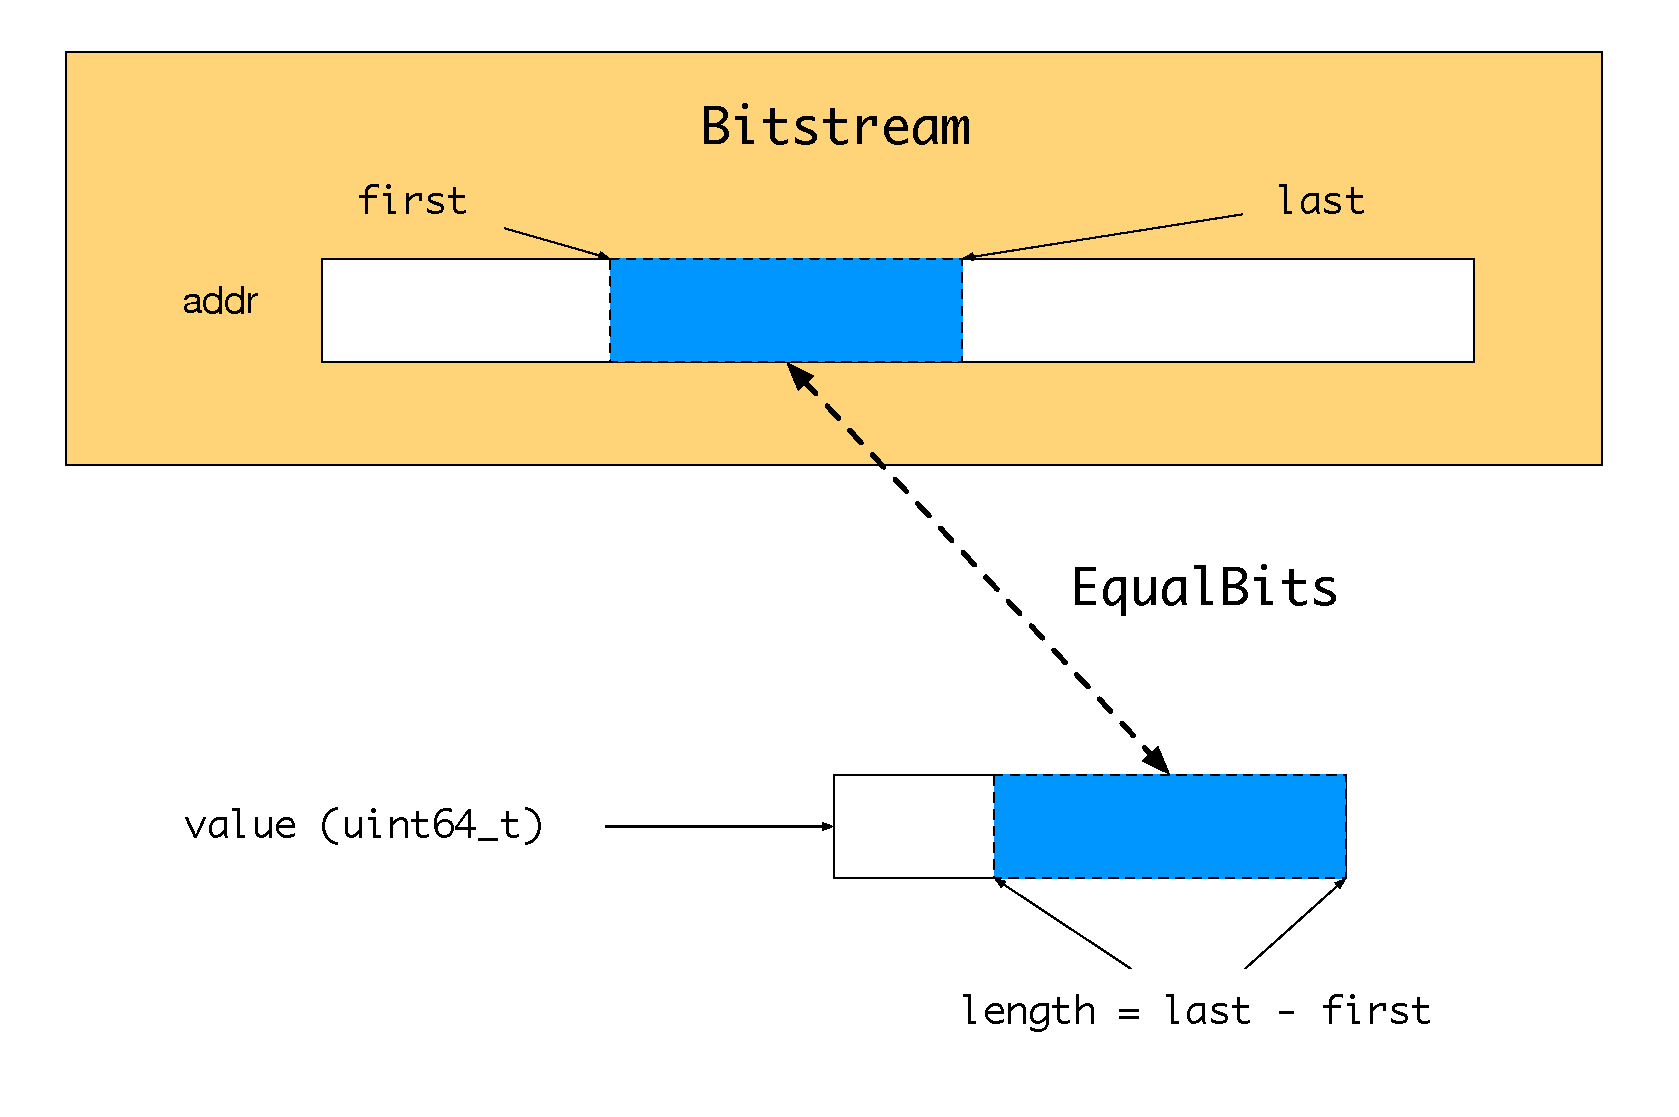
\includegraphics[width=0.99\textwidth]{figures/equalbits.pdf}
\caption{\label{fig:EqualBits correspondance}
	Bit coincidences required by \inl{EqualBits}}
\end{center}
\end{figure}



\FloatBarrier

\section{Auxiliary \inl{Bitstream} functions}
\label{sec:bitstream-aux}


As a kind of constructor for type
\inl{Bitstream}, we provide the operation \inl{Bitstream_Init},
shown with its contract in Listing~\ref{lst:Bitstream_Init}.




\begin{listing}[hbt]
\begin{minipage}{0.99\textwidth}
\begin{lstlisting}[style=acsl-block]
/*@
  requires valid:     Writeable(stream);
  requires bit_size:  8 * size <= UINT32_MAX;
  requires valid_pos: bitpos <= 8 * size;
  requires separated: \separated(addr + (0..size-1), stream);

  assigns  stream->addr, stream->size, stream->bitpos;

  ensures  addr:      stream->addr == addr;
  ensures  size:      stream->size == size;
  ensures  bitpos:    stream->bitpos == bitpos;
  ensures  invariant: Invariant(stream, 0);
*/
void Bitstream_Init(Bitstream* stream, uint8_t* addr, uint32_t size, uint32_t bitpos);
\end{lstlisting}
\end{minipage}
\caption{\label{lst:Bitstream_Init}Setting-up a bitstream}
\end{listing}

\FloatBarrier

Moreover, we provide a test for exhaustion of a \inl{Bitstream},
shown in Listing~\ref{lst:Bitstream_Normal}.


\begin{listing}[hbt]
\begin{minipage}{0.99\textwidth}
\begin{lstlisting}[style=acsl-block]
/*@
  requires valid:     Readable(stream);
  requires invariant: Invariant(stream, length);

  assigns \nothing;

  ensures  result:    \result <==> Normal(stream, length);
*/
int Bitstream_Normal(const Bitstream* stream, uint32_t length);
\end{lstlisting}
\end{minipage}
\caption{\label{lst:Bitstream_Normal}Testing a bitstream for exhaustion}
\end{listing}



\FloatBarrier


\section{Writing bit sequences}
\label{sec:writing bit sequences}

In this section, we describe the operations that handle plain bit sequences.
%
They are used to implement the \inl{Bitstream} operations for
Section~\ref{sec:bitstream}.

Listing~\ref{lst:Bitstream_Write impl} shows contract of
the \inl{Bitstream_Write} operation,
and moreover exemplifies its implementation.


\begin{listing}[hbt]
\begin{minipage}{0.99\textwidth}
\begin{lstlisting}[style=acsl-block]
/*@
  requires valid:      Writeable(stream);
  requires invariant:  Invariant(stream, length);
  requires normal:     Normal(stream, length);
  requires upper:      UpperBitsNotSet(value, length);

  assigns stream->addr[0..stream->size - 1];
  assigns stream->bitpos;

  ensures  pos:        stream->bitpos == \old(stream->bitpos) + length;
  ensures  changed:    EqualBits(stream, \old(stream->bitpos), stream->bitpos, value);
  ensures  unchanged:  Unchanged{Here,Old}(stream, 0, \old(stream->bitpos));
  ensures  unchanged:  Unchanged{Here,Old}(stream, stream->bitpos, 8 * stream->size);
  ensures  size:       stream->size == \old(stream->size);
*/
void Bitstream_Write(Bitstream* stream, uint32_t length, uint64_t value)
{
    Bitwalker_Write(stream->addr, stream->size, stream->bitpos, length, value);
    //@ assert EqualBits(stream, stream->bitpos, stream->bitpos + length, value);

    stream->bitpos += length;
    //@ assert EqualBits(stream, \at(stream->bitpos,Pre), stream->bitpos, value);
}

\end{lstlisting}
\end{minipage}
\caption{\label{lst:Bitstream_Write impl}Writing to a bitstream}
\end{listing}

\FloatBarrier

Most parts of the contract are quite similar to that of
\inl{Bitstream_Read} in
Listing~\ref{lst:Bitstream_Read spec}.
%
Differences are the following:
\begin{itemize}
\item We require that the \inl{value} to be written fits into
	the specified
	\inl{length}, i.e.\ its unused most significant bits
	are zero (requirement property
	``\inl{upper}'').
\item The operation is allowed to change the contents of the bitstream
	(first \inl{assigns} clause) in addition to the streams
	current bit
	position (second \inl{assigns} clause), but no other
	memory locations.
\item Since we couldn't specify in the \inl{assigns} clauses 
	which bits exactly are allowed to be modified, we give the
	details in two
	\inl{ensures} clauses named ``\inl{unchanged}'':
	All bits before the stream's \inl{bitpos} on operation
	entry, and after
	its \inl{bitpos} on exit, must remain unchanged.
\end{itemize}

The implementation just employs the lower-level operation
\inl{Bitwalker_Write} to
write the bits, and appropriately updates the \inl{stream}'s
\inl{bitpos}.
%
Two assertions were needed to help the provers establishing that
\inl{value}'s
bits are actually written to \inl{stream}'s data array by
\inl{Bitwalker_Write}, and that they aren't subsequently destroyed by
the increment of \inl{bitpos}.



The formal definitions of the used \acsl predicates are given in
Listing~\ref{lst:Bitsequence preds}.
%
Again, the tacit assumption that the array contains sensible data
up to its very last bit is used in predicate \inl{Normal}.



\begin{listing}[hbt]
\begin{minipage}{0.99\textwidth}
\begin{lstlisting}[style=acsl-block]
/*@
   predicate Readable{L}(uint8_t* addr, integer size) = \valid_read(addr + (0..size-1));

   predicate Writeable{L}(uint8_t* addr, integer size) = \valid(addr + (0..size-1));

   predicate Invariant{L}(integer size, integer bitpos, integer length) =
       8 * size <= UINT32_MAX         &&
       length <= 64                   &&
       bitpos + length <= UINT32_MAX;

    predicate Normal{L}(integer size, integer bitpos, integer length) =
       bitpos + length <= 8 * size;
*/
\end{lstlisting}
\end{minipage}
\caption{\label{lst:Bitsequence preds} \acsl predicates used in bit sequence layer contracts}
\end{listing}


\FloatBarrier


Listing~\ref{Bitwalker_Write spec} shows the contract, and the
implementation, of the
\inl{Bitwalker_Write} operation.

\begin{listing}[hbt]
\begin{minipage}{0.99\textwidth}
\begin{lstlisting}[style=acsl-block]
/*@
  requires valid:      Writeable(addr, size);
  requires invariant:  Invariant(size, bitpos, length);
  requires normal:     Normal(size, bitpos, length);
  requires upper:      UpperBitsNotSet(value, length);

  assigns addr[0..size-1];

  ensures  left:       Unchanged{Here,Old}(addr, 0, bitpos);
  ensures  middle:     EqualBits(addr, bitpos, bitpos + length, value);
  ensures  right:      Unchanged{Here,Old}(addr, bitpos + length, 8 * size);
*/
void Bitwalker_Write(uint8_t* addr, uint32_t size, uint32_t bitpos, uint32_t length, uint64_t value);
{
    /*@
      loop invariant bound:   bitpos <= i <= bitpos + length;
      loop invariant left:    Unchanged{Here,Pre}(addr, 0, bitpos);
      loop invariant middle:  EqualBits(addr, bitpos, i, value, length);
      loop invariant right:   Unchanged{Here,Pre}(addr, i, 8 * size);

      loop assigns  i, addr[0..size-1];
      loop variant  bitpos + length - i;
    */
    for (uint32_t i = bitpos; i < bitpos + length; ++i)
    {
        int flag = TestBit64(value, (64 - length) + (i - bitpos));
        SetBit8Array(addr, size, i, flag);
    }   
}

\end{lstlisting}
\end{minipage}
\caption{\label{Bitwalker_Write spec}Writing a bit sequence}
\end{listing}

\FloatBarrier

\section{Reading bit sequences}
\label{sec:reading bit sequences}

The following peculiarities are observed when the former is
compared to \inl{Bitwalker_Read}'s contract in Listing~\ref{lst:Bitwalker_Read spec}.

\begin{listing}[hbt]
\begin{minipage}{0.99\textwidth}
\begin{lstlisting}[style=acsl-block]
/*@
  requires  valid:      Readable(addr, size);
  requires  invariant:  Invariant(size, bitpos, length);
  requires  normal:     Normal(size, bitpos, length);

  assigns   \nothing;

  ensures   equal:      EqualBits(addr, bitpos, bitpos + length, \result);
  ensures   upper:      UpperBitsNotSet(\result, length);
*/
uint64_t Bitwalker_Read(uint8_t* addr, uint32_t size, uint32_t bitpos, uint32_t length);
\end{lstlisting}
\end{minipage}
\caption{\label{lst:Bitwalker_Read spec}Reading a bit sequence}
\end{listing}

\FloatBarrier

\begin{itemize}
\item We require that the \inl{value} to be written fits into
the specific
	\inl{length}, i.e.\ all but its \inl{length}
	least significant bits are
	zero (requirement property ``\inl{upper}'').
\item The operation may modify the data array at \inl{addr},
but nothing else.
\item Again, we give the details of which data bits exactly
	are allowed to be changed in two
	\inl{ensures} clauses, named ``\inl{left}'' and
	``\inl{right}'', and requiring all bits before
	\inl{bitpos} and after
	\inl{bitpos+length} to remain unchanged, respectively.
\end{itemize}

In the implementation, which is shown here as an example, we used
the straight-forward
algorithm that takes a bit from \inl{value} and places it into
the \inl{addr} array, bit by bit.
%
In order for the provers to establish that algorithm's correctness,
we had to provide a total of six \acsl clauses about the loop:
%
\begin{itemize}
\item The loop variable, \inl{i}, always ranges in the interval
	[\inl{bitpos}\ldots\inl{bitpos+length}]---loop invariant property ``\inl{bound}''.
	%
	Note that the highest value is actually taken,
	viz.\ on exit of the loop body in the last iteration,
	subsequently causing the loop to terminate.
\item The bits before \inl{bitpos}, and after
	\inl{bitpos+length}
	remain as they were on operation entry---invariant property
	``\inl{left}'' and ``\inl{right}'', respectively.
\item In the \inl{i}th iteration, the bits
	[\inl{bitpos}\ldots\inl{bitpos+i}) agree with
	the least significant
	\inl{i} bits of \inl{value}---invariant property
	``\inl{middle}''.
\item The loop code is allowed to modify the variable \inl{i},
	and the whole array
	at \inl{addr}, but nothing else---
	\inl{loop assigns} clause.
\item The value of the integer
	expression \inl{bitpos+length-i} is non-negative throughout
	the whole loop execution, but is decreased in every iteration 
	--- \inl{loop variant} clause.
	%
	Therefore, the loop is guaranteed to terminate eventually.
\end{itemize}




The operations we have discussed here are based
on operations to write and to read a single bit.
%
The details of the latter, as well as of the predicates used in their
contracts, are given in Chapter~\ref{cha:low-level bitstream}.

\FloatBarrier


\section{Verification of the Bitstream abstraction}
\label{sec:bitstream verif}



Critics of the formal software verification approach often 
argue that verifying an operation against its formal specification
results in little or no increase of trustworthiness when
%
\begin{itemize}
\item the specification, including all auxiliary definitions etc., is
	as complex as the operation's implementation, or/and
\item the specification essentially duplicates the implemented
	algorithm in a different (such as functional rather than
	imperative) language.
\end{itemize}
%
Both criteria may be seen to be met by our Bitwalker case study.



However, since the operations we dealt with essentially implement a
communication protocol, there is a very simple ``high-level'' property
that should be satisfied, viz.\ that a ``send'' operation is inverse
to a ``receive'' operation.
%
This property can be stated formally in a very brief and understandable
way.
%
It ensures, in a mathematical context, that both operations implement
bijective mappings, that is, in an engineering sense, that the
communication channel neither looses, nor subjoins information.
%
In fact, we have achieved to formally prove this property.




More particularly, in our setting, we could show that the operations
\inl{Bitstream_Read} and \inl{Bitstream_Write} are
inverse to each other.
%
To this end, we set up two fictitious \isoc procedures realizing
the composition of both operations in the two possible orders.




Listing~\ref{lst:Bitstream_WriteThenRead}
shows the procedure for the scenario ``use \inl{Bitstream_Write}
to write a value to a stream, then immediately read it back using
\inl{Bitstream_Read}''.


\begin{listing}[hbt]
\begin{minipage}{0.99\textwidth}
\begin{lstlisting}[style=acsl-block]
/*@
    requires valid:      Writeable(stream);
    requires invariant:  Invariant(stream, length);
    requires normal:     Normal(stream, length);
    requires upper:      UpperBitsNotSet(value, length);

    assigns stream->addr[0..stream->size-1];
    assigns stream->bitpos;

    ensures equality:     \result == value;
*/
uint64_t Bitstream_WriteThenRead(Bitstream* stream, uint32_t length, uint64_t v>
{
    //@ ghost uint32_t old_pos = stream->bitpos;

    Bitstream_Write(stream, length, value);
    //@ assert equal:  EqualBits(stream, old_pos, old_pos+length, value);

    /*@ 
        assigns stream->bitpos;
        ensures reset: stream->bitpos == \at(stream->bitpos,Pre);
    */
    stream->bitpos -= length;

    uint64_t result = Bitstream_Read(stream, length);
    //@ ghost uint32_t new_pos = stream->bitpos;
    //@ assert equal_result: EqualBits(stream, old_pos, new_pos, result);
    //@ assert equal_value:  EqualBits(stream, old_pos, new_pos, value);
    /*@ assert aux:          \forall integer k; old_pos <= k < new_pos ==>
                               \let j = new_pos - 1 - k;
                               (BitTest(value,  j) <==> BitTest(result, j));
    */
    //@ assert left:         EqualBits64(result, value, 64-length, 64);
    //@ assert compare:      EqualBits64(result, value, 0, 64);

    return result;
}
\end{lstlisting}
\end{minipage}
\caption{\label{lst:Bitstream_WriteThenRead}
	Verifying the scenario ``write, then read'' }
\end{listing}

\FloatBarrier

The procedure's body code is straightforward; after
\inl{Bitstream_Write}, we have to seek back to the original bit
position, before calling \inl{Bitstream_Read}''.
%
We could show that the read value always equals the written one,
provided
\begin{itemize}
\item the stream is accessible for both read and update
	(requirement property ``\inl{valid}''),
\item it satisfies its type invariant (property
	``\inl{invariant}''; cf.\ Listing~\ref{lst:Bitstream preds}
	and~\ref{lst:Bitsequence preds}),
\item the stream's current bit position is sufficiently small such that
	all value bits still fit into the stream
	(property``\inl{normal}''), and
\item the most significant value bits that are not written are all zero
	(property``\inl{upper}'').
\end{itemize}
%
This ensures that the bitstream communication channel doesn't loose
information---every value we write into it can completely be
restored.



Vice versa, we could also show that the channel doesn't transmit more
information than is needed to fulfill its task.
%
Listing~\ref{lst:Bitstream_ReadThenWrite}
shows the procedure for the scenario ``use \inl{Bitstream_Read}
to read a value from a stream, then immediately write it back using
\inl{Bitstream_Write}''.




\begin{listing}[hbt]
\begin{minipage}{0.99\textwidth}
\begin{lstlisting}[style=acsl-block]
/*@
    requires valid:      Writeable(stream);
    requires invariant:  Invariant(stream, length);
    requires normal:     Normal(stream, length);

    assigns stream->addr[0..stream->size-1];
    assigns stream->bitpos;

    ensures  unchanged:  Unchanged{Here,Old}(stream, 0, 8 * stream->size);
*/
void Bitstream_ReadThenWrite(Bitstream* stream, uint32_t length)
{
    //@ ghost uint32_t old_pos = stream->bitpos;
    uint64_t value = Bitstream_Read(stream, length);
    //@ assert equal:  EqualBits(stream, old_pos, old_pos+length, value);

    stream->bitpos -= length;
    //@ assert stream->bitpos == old_pos;

    Bitstream_Write(stream, length, value);
    //@ assert unchanged:  Unchanged{Here,Pre}(stream, old_pos, stream->bitpos);
}
\end{lstlisting}
\end{minipage}
\caption{\label{lst:Bitstream_ReadThenWrite}
	Verifying the scenario ``read, then write'' }
\end{listing}


\FloatBarrier


We were able show that this leaves the
whole stream unchanged, provided the first three requirement properties
from \inl{Bitstream_WriteThenRead} are met.
%
As an example for a channel transmitting redundant information,
consider
a bitstream implementation
with \inl{Bitstream_Write}
storing each byte twice in succession and \inl{Bitstream_Read}
ignoring every second byte.
%
Such a stream doesn't meet our property, since, 
starting from a stream with non-agreeing adjacent bytes, there is no
way to reproduce it by a ``read, then write'' scenario.

